\documentclass[border=4pt]{standalone}
\usepackage{mathptmx}
\usepackage{tabularx}
\usepackage{caption}
\usepackage{booktabs}
\usepackage{amsmath, amssymb, amsthm}
\usepackage[hidelinks]{hyperref}
\usepackage{tikz}
\usetikzlibrary{shapes.geometric,arrows.meta,positioning,calc,shadows}
\usepackage{xcolor}
\usepackage{array}
\usepackage{makecell}   % \makecell[l]{a\\b} = wrap a table cell onto several lines
\usepackage{enumitem}   % tight list spacing (see the contributions list in Sec 1)
\usepackage{float}   % [H] = pin a figure/table exactly here (no floating to page bottom)
\definecolor{predblue}{HTML}{1D6FE0}
\definecolor{execred}{HTML}{E63946}
\newcommand{\legdot}{\tikz[baseline=-0.5ex]\draw[predblue,fill=predblue] (0,0) circle (2.2pt);}
\newcommand{\legx}{\tikz[baseline=-0.5ex]{\draw[execred,line width=1.2pt] (-2.1pt,-2.1pt)--(2.1pt,2.1pt);\draw[execred,line width=1.2pt] (-2.1pt,2.1pt)--(2.1pt,-2.1pt);}}
\newcommand{\legarrow}{\tikz[baseline=-0.4ex]\draw[gray,line width=1.2pt,-{Latex[length=3pt]}] (0,0)--(10pt,0);}
\definecolor{routebrown}{HTML}{7A3B00}
\newcommand{\legroute}{\tikz[baseline=-0.4ex]\draw[routebrown,line width=1.6pt,-{Triangle[length=4pt,width=4pt]}] (0,0)--(11pt,0);}
\definecolor{cushblue}{HTML}{1D6FE0}
\definecolor{oraclepurple}{HTML}{7C3AED}
\definecolor{devamber}{HTML}{E39E14}   % deviant agent, matches plots/jul28/generators/bar_style.py
\definecolor{diagLaw}{HTML}{1D6FE0}
\definecolor{diagPlan}{HTML}{E63946}
\definecolor{diagEnv}{HTML}{12A150}
\definecolor{diagLatent}{HTML}{7C3AED}
\definecolor{diagProbe}{HTML}{E8890C}
\definecolor{gapblue}{HTML}{00B4D8}   % grounding gap: bright cyan, outside the node palette
\definecolor{gapred}{HTML}{C2185B}    % ontological gap: magenta. Teal/magenta stay distinct under deuteranopia.
\newcommand{\cushsoc}{\tikz[baseline=-0.35ex]\draw[cushblue,line width=1.7pt] (0,0)--(11pt,0);}
\newcommand{\cushora}{\tikz[baseline=-0.35ex]\draw[oraclepurple,line width=1.7pt] (0,0)--(11pt,0);}
\definecolor{agreal}{HTML}{E63946}
\definecolor{agsoc}{HTML}{1D6FE0}
\definecolor{agdev}{HTML}{E39E14}
\newcommand{\swatch}[1]{\tikz[baseline=-0.45ex]\draw[#1,fill=#1,rounded corners=0.4pt] (0,-2.6pt) rectangle (6.4pt,2.6pt);}
\newcommand{\agreal}{\swatch{agreal}}
\newcommand{\agsoc}{\swatch{agsoc}}
\newcommand{\agdev}{\swatch{agdev}}
\newcommand{\agora}{\swatch{oraclepurple}}
\usepackage[T1]{fontenc}
\usetikzlibrary{shadows.blur,shadows}
\begin{document}
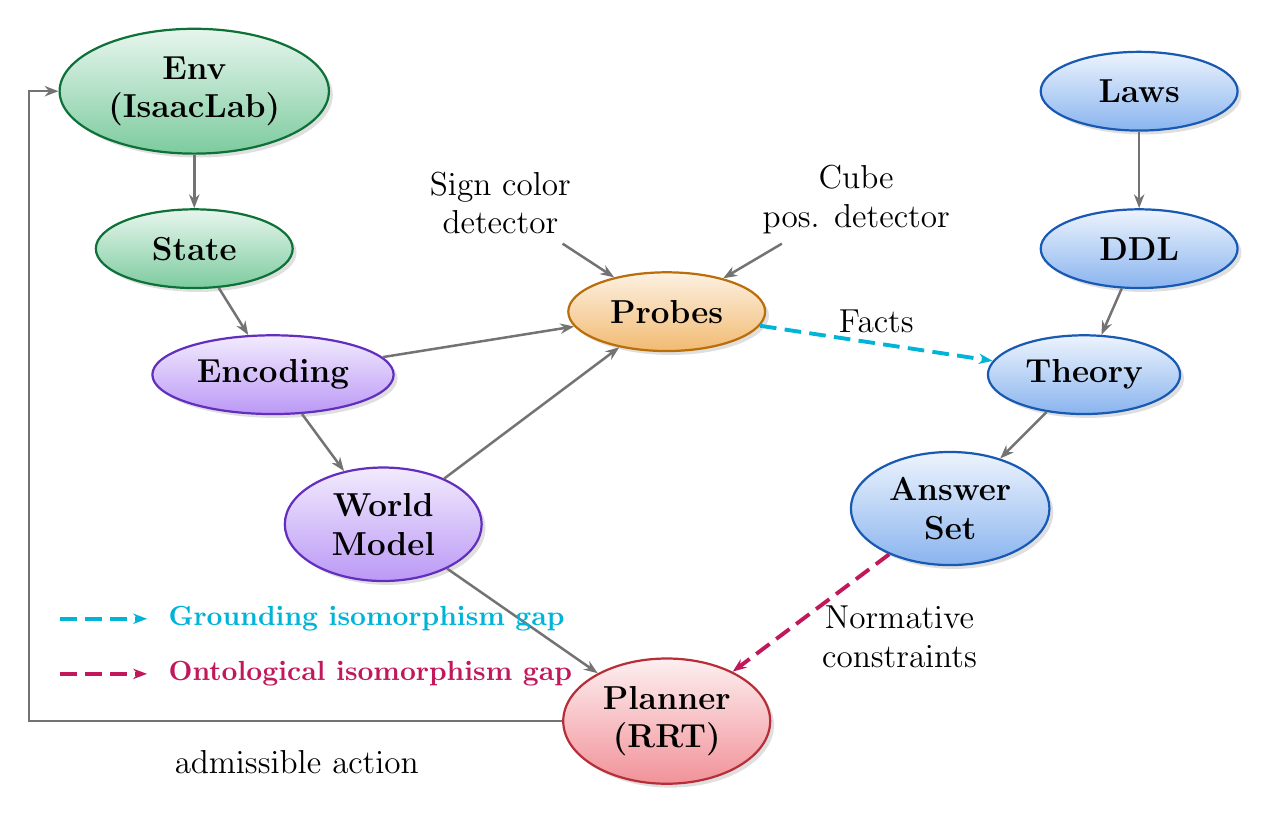
\begin{tikzpicture}[
            xshift=-2cm,
            >=Stealth,
            every node/.style={font=\large},
            box/.style={
                draw,
                line width=0.8pt,
                ellipse,
                minimum width=2.5cm,
                minimum height=1cm,
                align=center,
                font=\large\bfseries,
                drop shadow={shadow xshift=1.4pt, shadow yshift=-1.4pt, opacity=0.25}
            },
            envbox/.style={box, top color=diagEnv!10!white, bottom color=diagEnv!55, draw=diagEnv!70!black},
            latentbox/.style={box, top color=diagLatent!10!white, bottom color=diagLatent!52, draw=diagLatent!80!black},
            probebox/.style={box, draw=diagProbe!80!black, top color=diagProbe!12!white, bottom color=diagProbe!58},
            logicbox/.style={box, draw=diagLaw!80!black, top color=diagLaw!8!white, bottom color=diagLaw!52},
            plannerbox/.style={box, draw=diagPlan!80!black, top color=diagPlan!8!white, bottom color=diagPlan!55},
            arrow/.style={-{Stealth[length=5pt]}, line width=0.9pt, draw=black!55},
            % The two isomorphism gaps, drawn ON the arrows they afflict rather than as callouts.
            gapground/.style={-{Stealth[length=5pt]}, line width=1.4pt, draw=gapblue,
                              dash pattern=on 6pt off 3pt},
            gaponto/.style={-{Stealth[length=5pt]}, line width=1.4pt, draw=gapred,
                            dash pattern=on 6pt off 3pt}
        ]
        
        %---------------- Left ----------------%
        \node[envbox] (env) at (-6,2.8) {Env\\(IsaacLab)};
        \node[envbox] (state) at (-6,0.8) {State};
        \node[latentbox] (enc) at (-5,-0.8) {Encoding};
        \node[latentbox] (wm) at (-3.6,-2.7) {World\\Model};
        
        %---------------- Center ----------------%
        \node[probebox] (probes) at (0,0.0) {Probes};
        
        %---------------- Right reasoning pipeline ----------------%
        \node[logicbox] (db) at (6,2.8) {Laws};
        \node[logicbox] (ddl) at (6,0.8) {DDL};
        
        \node[logicbox, minimum width=2.1cm] (theory) at (5.3,-0.8) {Theory};
        \node[logicbox, minimum width=2.4cm] (answer) at (3.6,-2.5) {Answer\\Set};
        
        
        %---------------- Bottom ----------------%
        \node[plannerbox] (planner) at (0,-5.2) {Planner\\(RRT)};
        
        %================ Left pipeline =================%
        \draw[arrow] (env) -- (state);
        \draw[arrow] (state) -- (enc);
        \draw[arrow] (enc) -- (wm);
        
        %================ Converge to probes =================%
        \draw[arrow] (enc) -- (probes);
        \draw[arrow] (wm) -- (probes);
        
        %================ Right reasoning pipeline =================%
        \draw[arrow] (db) -- (ddl);
        \draw[arrow] (ddl) -- (theory);
        \draw[arrow] (theory) -- (answer);
        \draw[gaponto] (answer) -- node[midway, right, yshift=-0.3cm, align=center] {Normative \\constraints} (planner);
        
        % probes enter theory
        \draw[gapground] (probes) -- node[midway, above] {Facts} (theory);
        
        %================ Planner inputs =================%
        \draw[arrow] (wm) -- (planner);

        %================ Closed loop (absorbed from the old fig:loop) =================%
        \draw[arrow]
            (planner.west) -- (-8.1,-5.2) -- (-8.1,2.8) -- (env.west);
        \node[align=center, anchor=north] at (-4.7,-5.45) {admissible action};
        
        %================ Probe labels =================%
        \node[above right=0.5cm and 0.2cm of probes, align=center] (cubepos) {Cube\\pos. detector};
        \node[above left=0.5cm and 0.2
        cm of probes, align=center] (syncolor) {Sign color\\detector};
        
        \draw[arrow] (cubepos) -- (probes);
        \draw[arrow] (syncolor) -- (probes);

        %======= Legend for the two gaps (the arrows above carry the colour) =======%
        \draw[gapground] (-7.7,-3.9) -- (-6.6,-3.9);
        \node[right, font=\normalsize\bfseries, text=gapblue] at (-6.45,-3.9)
              {Grounding isomorphism gap};
        \draw[gaponto] (-7.7,-4.6) -- (-6.6,-4.6);
        \node[right, font=\normalsize\bfseries, text=gapred] at (-6.45,-4.6)
              {Ontological isomorphism gap};

        \end{tikzpicture}
\end{document}
